\documentclass[journal]{IEEEtran}

\usepackage{graphicx}
\usepackage{diagbox}
\usepackage{changepage}
\newcommand{\var}{\textit}
\newcommand{\proc}{\textbf}
\newcommand{\prop}{\texttt}
\newcommand{\plusplus}{{+}{+}}% Other options: 
\newcommand*\ita[1]{\textit{#1}}
\usepackage{array, booktabs, makecell, multirow}% new
\usepackage{textcomp}
\usepackage[dvipsnames,  x11names, table]{} % add more colors
\usepackage{tikz} % for the cup sketch
% \usepackage{ctable}% http://ctan.org/pkg/ctable
\usepackage{lettrine} % big letter in Intro

\usepackage{siunitx}
\sisetup{per=slash, load=abbr}
\usepackage{tikz}
\usepackage{pgfplots}
\pgfplotsset{width=7cm,compat=1.3}
\pgfplotsset{compat=1.12}
\usepgfplotslibrary{fillbetween} 
\usepgflibrary{shadings}
\usetikzlibrary{backgrounds}
\usetikzlibrary{fit,shapes.geometric}% <--- added

\definecolor{Gray}{gray}{0.9}
\definecolor{Green}{rgb}{0.0, 0.5, 0.0}
\definecolor{Yellow}{rgb}{0.85, 0.65, 0.13}
\definecolor{Grey}{rgb}{0.7, 0.7, 0.7}


% *** GRAPHICS RELATED PACKAGES ***
%
\ifCLASSINFOpdf
  % \usepackage[pdftex]{graphicx}
  % declare the path(s) where your graphic files are
  % \graphicspath{{../pdf/}{../jpeg/}}
  % and their extensions so you won't have to specify these with
  % every instance of \includegraphics
  % \DeclareGraphicsExtensions{.pdf,.jpeg,.png}
\else
  % or other class option (dvipsone, dvipdf, if not using dvips). graphicx
  % will default to the driver specified in the system graphics.cfg if no
  % driver is specified.
  % \usepackage[dvips]{graphicx}
  % declare the path(s) where your graphic files are
  % \graphicspath{{../eps/}}
  % and their extensions so you won't have to specify these with
  % every instance of \includegraphics
  % \DeclareGraphicsExtensions{.eps}
\fi

\begin{document}
%

\title{Detection of Object Properties from Human-Human Handover Actions and Applications in Robotics}
%
\author{Nuno Ferreira Duarte$^{1,2}$, 
        Aude Billard$^2$, and 
        Jos\'{e} Santos-Victor$^{1}$ 
        
\thanks{Corresponding author: Nuno Ferreira Duarte.}
\thanks{This work was partially supported by the RBCog-Lab research infrastructure, Funda\c{c}\~{a}o para a Ci\^{e}ncia e a Tecnologia (FCT) with reference UID/EEA/50009/2019, and the PhD grant with reference PD/BD/135116/2017 of Nuno Ferreira Duarte.}
\thanks{$^{1}$Vislab, Institute for Systems and Robotics, Instituto Superior T\'{e}cnico, Universidade de Lisboa, Portugal.
{\tt\{nferreiraduarte, jasv\}@isr.tecnico.ulisboa.pt}}

\thanks{$^2$LASA, Swiss Federal Institute of Technology, Lausanne, Switzerland. {\tt \{nuno.ferreiraduarte, aude.billard\}@epfl.ch.}}
}

% The paper headers
\markboth{IEEE ROBOTICS AND AUTOMATION LETTERS, ~Vol.~?, No.~?, Apri~2021}%
{Shell \MakeLowercase{\textit{et al.}}: Bare Demo of IEEEtran.cls for IEEE Journals}
% The only time the second header will appear is for the odd numbered pages
% after the title page when using the twoside option.
% 
% *** Note that you probably will NOT want to include the author's ***
% *** name in the headers of peer review papers.                   ***
% You can use \ifCLASSOPTIONpeerreview for conditional compilation here if
% you desire.

% If you want to put a publisher's ID mark on the page you can do it like
% this:
%\IEEEpubid{0000--0000/00\$00.00~\copyright~2015 IEEE}
% Remember, if you use this you must call \IEEEpubidadjcol in the second
% column for its text to clear the IEEEpubid mark.


% make the title area
\maketitle

\begin{abstract}

% witty, interesting take on robotics, and human interactions
Robots can learn a lot from humans interacting amidst each other as well as objects. Humans when interacting with objects reveal, through their non-verbal communication, extrinsic properties of said objects. Our aim is to develop controllers that use this information to aid robots during manipulation of unknown objects.

% contributions 
To achieve this, first, we analyse the kinematic motion of the human arm during handovers of cups and glasses under two conditions: (i) empty, and (ii) filled with water. From the kinematic motion, it was recognized two distinct strategies according to the human perceived challenge: (i) unrestricted, free motion - natural manipulation; and (ii) constrained, challenging motion due to danger of spilling - careful manipulation. Secondly, we compare two computational model approaches that aim to describe the two kinematic strategies observed: (i) deceleration phase, and (ii) acceleration phase. Thirdly, from the approach with the best results, we embedded the model in a robot controller with a human-in-the-loop where the approach is tested on human-object interaction and human-robot interaction scenarios. 

The results show that the acceleration phase approach can generalize well to unknown people, cups, and new human handover scenarios (datasets). The robot controller proves that it can be applied to multiple human-robot tasks and provide accurate information on the object properties or human motion preference. 

\end{abstract}

% Note that keywords are not normally used for peerreview papers.
% \begin{IEEEkeywords}
% IEEE, IEEEtran, journal, \LaTeX, paper, template.
% \end{IEEEkeywords}

%%%%%%%%%%%%%%%%%%%%%%%%%%%
\section{Introduction}

what you talk about:

- in the intro you introduce the idea, the challenge, the different ways that people have tried to use to solve it, and your proposal
- you mention the CV people who are trying to detect liquid levels or if the cup has liquid or not from images or videos. There is a problem with occlusions, different types of cups, color of cups, opaque cups (where it is impossible to tell). I propose another way that helps solve that problem

\input{2_analysis.tex}
\input{3_model.tex}
\section{Experimental Results} \label{sec:results}

\subsection{Results for different cups}

\begin{table} 
\centering 
\resizebox{\columnwidth}{!}{%
\begin{tabular}{l l c c c c c c} 
\toprule % Top horizontal line
 & & & \multicolumn{5}{c}{\textbf{Acceleration Approach}} \\ 
\cmidrule(l){4-7} 
\textbf{Type of Cup} &  &  & \multicolumn{2}{c}{Training Set} & \multicolumn{2}{c}{Testing Set} &\\ % Column names row
\cmidrule(l){4-7} 
\textbf{Train} & \textbf{Test} & \diagbox{Predicted}{Real} & Empty & Full & Empty & Full &\\ % Column names row
\midrule % In-table horizontal line

 & \textcolor{Yellow}{Red Cup}  & \multirow{2}{*}{Not Careful}  & \multirow{2}{*}{0.688} & \multirow{2}{*}{\textcolor{Grey}{0.15}} & \multirow{2}{*}{\textbf{0.46}} & \multirow{2}{*}{\textcolor{Grey}{0.1}} \\ %
\textcolor{Yellow}{Transparent Cup} & \textcolor{Yellow}{Champagne} & \multirow{2}{*}{ Careful} & \multirow{2}{*}{\textcolor{Grey}{0.312}} &  \multirow{2}{*}{0.85} & \multirow{2}{*}{\textcolor{Grey}{0.54}} & \multirow{2}{*}{\textbf{0.90}} \\ 
 & \textcolor{Green}{Wine Glass} & & & & & \\ % 
 
 \cmidrule(l){2-7} 
 & \textcolor{Yellow}{Transparent Cup} & & \multirow{2}{*}{0.5} & \multirow{2}{*}{\textcolor{Grey}{0.1}} & \multirow{2}{*}{\textbf{0.53}} & \multirow{2}{*}{\textcolor{Grey}{0.15}} \\ % 
\textcolor{Yellow}{Champagne} & \textcolor{Yellow}{Red Cup} & & \multirow{2}{*}{\textcolor{Grey}{0.5}} & \multirow{2}{*}{0.9} & \multirow{2}{*}{\textcolor{Grey}{0.47}} & \multirow{2}{*}{\textbf{0.85}}\\ % 
 & \textcolor{Green}{Wine Glass} &  & &  &  & \\ % 
 
 \cmidrule(l){2-7} 
 & \textcolor{Yellow}{Transparent Cup} & & \multirow{2}{*}{0.47} & \multirow{2}{*}{\textcolor{Grey}{0}} & \multirow{2}{*}{\textbf{0.5}} & \multirow{2}{*}{\textcolor{Grey}{0.16}} \\ % 
\textcolor{Yellow}{Red Cup} & \textcolor{Yellow}{Champagne} & & \multirow{2}{*}{\textcolor{Grey}{0.53}} & \multirow{2}{*}{1} & \multirow{2}{*}{\textcolor{Grey}{0.5}} & \multirow{2}{*}{\textbf{0.84}}\\ % 
 & \textcolor{Green}{Wine Glass} &  & &  &  & \\ % 
 
 \cmidrule(l){2-7} 
 & \textcolor{Yellow}{Transparent Cup} & & \multirow{2}{*}{0.5} & \multirow{2}{*}{\textcolor{Grey}{0.25}} & \multirow{2}{*}{\textbf{0.59}} & \multirow{2}{*}{\textcolor{Grey}{0.17}}\\ % 
\textcolor{Green}{Wine Glass} & \textcolor{Yellow}{Red Cup} & & \multirow{2}{*}{\textcolor{Grey}{0.5}} & \multirow{2}{*}{0.75} & \multirow{2}{*}{\textcolor{Grey}{0.41}} & \multirow{2}{*}{\textbf{0.83}}\\ % 
 & \textcolor{Yellow}{Champagne} & &  &  &  & \\ % 
 
  \cmidrule(l){2-7} 
 & \textcolor{Yellow}{Red Cup} & & \multirow{2}{*}{0.688} & \multirow{2}{*}{\textcolor{Grey}{0.15}} & \multirow{2}{*}{\textbf{0.52}} & \multirow{2}{*}{\textcolor{Grey}{0.04}} \\
\textcolor{Yellow}{Transparent Cup} & & & \multirow{2}{*}{\textcolor{Grey}{0.312}} & \multirow{2}{*}{0.85} & \multirow{2}{*}{\textcolor{Grey}{0.48}} & \multirow{2}{*}{\textbf{0.96}}\\ % 
 & \textcolor{Yellow}{Champagne} &  & &  &  &  \\ % 
 
  \cmidrule(l){2-7} 
 & \textcolor{Yellow}{Transparent Cup} & & \multirow{2}{*}{0.5} & \multirow{2}{*}{\textcolor{Grey}{0.1}} & \multirow{2}{*}{\textbf{0.55}} & \multirow{2}{*}{\textcolor{Grey}{0.08}} \\ % 
\textcolor{Yellow}{Champagne} &  & & \multirow{2}{*}{\textcolor{Grey}{0.5}} & \multirow{2}{*}{0.9} & \multirow{2}{*}{\textcolor{Grey}{0.45}} & \multirow{2}{*}{\textbf{0.92}}\\ %
 & \textcolor{Yellow}{Red Cup} & &  &  &  & \\ %   
 
  \cmidrule(l){2-7} 
 & \textcolor{Yellow}{Transparent Cup} & & \multirow{2}{*}{0.47} & \multirow{2}{*}{\textcolor{Grey}{0}} & \multirow{2}{*}{\textbf{0.5}} & \multirow{2}{*}{\textcolor{Grey}{0.09}} \\ % 
\textcolor{Yellow}{Red Cup} &  & & \multirow{2}{*}{\textcolor{Grey}{0.53}} & \multirow{2}{*}{1} & \multirow{2}{*}{\textcolor{Grey}{0.5}} &  \multirow{2}{*}{\textbf{0.91}}\\ % 
 & \textcolor{Yellow}{Champagne} &  &  &  & \\ % 
 
  \cmidrule(l){2-7} 
\textcolor{Yellow}{Transparent Cup}  &  & & \multirow{2}{*}{0.61} & \multirow{2}{*}{\textcolor{Grey}{0.15}} & \multirow{2}{*}{\textbf{0.625}} & \multirow{2}{*}{\textcolor{Grey}{0.3}} \\ % 
 & \textcolor{Yellow}{Champagne}  & & \multirow{2}{*}{\textcolor{Grey}{0.39}} & \multirow{2}{*}{0.85} & \multirow{2}{*}{\textcolor{Grey}{0.375}} &  \multirow{2}{*}{\textbf{0.7}}\\ % 
\textcolor{Yellow}{Red Cup}  & &  &  &  & \\ % 
 
\midrule % In-table horizontal line
\midrule % In-table horizontal line
\end{tabular}
}
\caption{One vs Rest Classification. Training set: One cup type; Testing set: Other cup types. \textcolor{Yellow}{Plastic cups}; \textcolor{Green}{Glass cups}}
\label{tab:one_vs_all} 
\end{table}

Conclusions from Table \ref{tab:one_vs_all}:
Training on one plastic and testing on the rest: 86\% $\pm$ 2.9\% Full cups are Careful, 49.6\% $\pm$ 2.9\% Empty cups are NOT Careful. Training on one plastic and testing on other plastics: 93\% $\pm$ 2.2\% Full cups are Careful, 52\% $\pm$ 2.1\% Empty cups are NOT Careful. Training on glass and testing on plastics: 83\% Full cups are Careful,	59\% Empty cups are NOT Careful.

Soft plastics vs Rigid plastics: 70\% vs 92\% for Full cups are Careful, 63\% vs 55\% for Empty cups are NOT Careful. 

The classifier predicts that unknown Full cups are predominantly classified as Careful manipulations irrespective of the type of cup the model is trained on.
Training and testing on plastics achieves the best results since it induces similar characteristics (e.g. risk of breaking, friction, weight, etc.) 
Training a model on glass and testing on plastics worsens the likelihood of detecting Full cups as Careful manipulations which could be induced by different characteristics being present (glass can break, and glass is heavier than plastic)
Soft plastics vs Rigid plastics: 		
Soft is difficult to handle when full of water, deformable;
Rigid plastic is closer to a glass, not deformable; 
A model trained on soft plastics learns that Full cups actions are extremely difficult, hence Full cups actions for Rigid plastics have a higher tendency to be classified NOT Careful.
A model trained on Rigid plastics learns the opposite hence Full cups actions for soft plastics are mostly classified as Careful manipulations

\subsection{Results for different datasets}

- DONT FORGET TO PRESENT THE DATASETS (SUCCINCTLY) \cite{xompero_corsmal_2020} 
%%%%% EPFL vs EPFL (rest) dataset %%%%%%%%%%%%

\begin{table} 
\centering 
\resizebox{\columnwidth}{!}{%
\begin{tabular}{l l c c c c c c} 
\toprule % Top horizontal line
 & & & \multicolumn{5}{c}{\textbf{Acceleration Approach}} \\ 
\cmidrule(l){4-7} 
\textbf{} &  &  & \multicolumn{2}{c}{Training Set} & \multicolumn{2}{c}{Testing Set} &\\ % Column names row
\cmidrule(l){4-7} 
\textbf{Train} & \textbf{Test} & \diagbox{Predicted}{Real} & Empty & Full & Empty & Full &\\ % Column names row
\midrule % In-table horizontal line

\multirow{2}{*}{EPFL 10\%}  & \multirow{2}{*}{EPFL 90\%} & Not Careful & 0.83 & \textcolor{Grey}{0} & \textbf{0.53} &  \textcolor{Grey}{0.19}\\
  &   & Careful & \textcolor{Grey}{0.17} & 1 & \textcolor{Grey}{0.47} & \textbf{0.81} \\
  
  \cmidrule(l){2-7} 
\multirow{2}{*}{EPFL 20\%}  & \multirow{2}{*}{EPFL 80\%} &  & 0.89 & \textcolor{Grey}{0.12} & \textbf{0.5} &  \textcolor{Grey}{0.16}\\
  &   &  & \textcolor{Grey}{0.11} & 0.88 & \textcolor{Grey}{0.5} & \textbf{0.84}  \\ 
  
\cmidrule(l){2-7} 
\multirow{2}{*}{EPFL 30\%}  & \multirow{2}{*}{EPFL 70\%} &  & 0.69 & \textcolor{Grey}{0.09} & \textbf{0.51} &  \textcolor{Grey}{0.15}\\
  &   &  & \textcolor{Grey}{0.31} & 0.91 & \textcolor{Grey}{0.15} & \textbf{0.85}  \\
  
\cmidrule(l){2-7} 
\multirow{2}{*}{EPFL 40\%}  & \multirow{2}{*}{EPFL 60\%} &  & 0.6 & \textcolor{Grey}{0.13} & \textbf{0.55} &  \textcolor{Grey}{0.1}\\
  &   &  & \textcolor{Grey}{0.4} & 0.87 & \textcolor{Grey}{0.45} & \textbf{0.9}  \\

\cmidrule(l){2-7} 
\multirow{2}{*}{EPFL 50\%}  & \multirow{2}{*}{EPFL 50\%} &  & 0.61 & \textcolor{Grey}{0.16} & \textbf{0.5} &  \textcolor{Grey}{0.1}\\
  &   &  & \textcolor{Grey}{0.39} & 0.84 & \textcolor{Grey}{0.5} & \textbf{0.9}  \\
  
\cmidrule(l){2-7} 
\multirow{2}{*}{EPFL 60\%}  & \multirow{2}{*}{EPFL 40\%} &  & 0.55 & \textcolor{Grey}{0.08} & \textbf{0.5} &  \textcolor{Grey}{0.15}\\
  &   &  & \textcolor{Grey}{0.45} & 0.92 & \textcolor{Grey}{0.5} & \textbf{0.85}  \\
  
  
\midrule % In-table horizontal line
\midrule % In-table horizontal line
\end{tabular}
}
\label{tab:epfl} % A label for referencing this table elsewhere, references are used in text as \ref{label}
\caption{Training set: small size of the EPFL dataset; Testing set: the rest of the EPFL dataset.}
\end{table}

%%%%% QMUL dataset %%%%%%%%%%%%

\begin{table} 
\centering 
\resizebox{\columnwidth}{!}{%
\begin{tabular}{l l c c c c c c} 
\toprule % Top horizontal line
 & & & \multicolumn{5}{c}{\textbf{Acceleration Approach}} \\ 
\cmidrule(l){4-7} 
\textbf{} &  &  & \multicolumn{2}{c}{Training Set} & \multicolumn{2}{c}{Testing Set} &\\ % Column names row
\cmidrule(l){4-7} 
\textbf{Train} & \textbf{Test} & \diagbox{Predicted}{Real} & Empty & Full & Empty & Full &\\ % Column names row
\midrule % In-table horizontal line

\multirow{2}{*}{EPFL 10\%}  & \multirow{1}{*}{QMUL} & Not Careful & 1 & \textcolor{Grey}{0} & \textbf{0.5625} &  \textcolor{Grey}{0.2}\\
  &   & Careful & \textcolor{Grey}{0} & 1 & \textcolor{Grey}{0.4375} & \textbf{0.8} \\
  
  \cmidrule(l){2-7} 
\multirow{2}{*}{EPFL 20\%}  & \multirow{1}{*}{QMUL} &  & 0.92 & \textcolor{Grey}{0.14} & \textbf{0.5} &  \textcolor{Grey}{0.2}\\
  &   &  & \textcolor{Grey}{0.08} & 0.86 & \textcolor{Grey}{0.5} & \textbf{0.8}  \\ 
  
\cmidrule(l){2-7} 
\multirow{2}{*}{EPFL 40\%}  & \multirow{1}{*}{QMUL} &  & 0.94 & \textcolor{Grey}{0.18} & \textbf{0.5} &  \textcolor{Grey}{0.13}\\
  &   &  & \textcolor{Grey}{0.06} & 0.82 & \textcolor{Grey}{0.5} & \textbf{0.87}  \\
  
\cmidrule(l){2-7} 
\multirow{2}{*}{EPFL 50\%}  & \multirow{1}{*}{QMUL} &  & 0.7 & \textcolor{Grey}{0.29} & \textbf{0.5} &  \textcolor{Grey}{0.27}\\
  &   &  & \textcolor{Grey}{0.3} & 0.71 & \textcolor{Grey}{0.5} & \textbf{0.73}  \\
  
\midrule % In-table horizontal line
\midrule % In-table horizontal line
\end{tabular}
}
\caption{Classifier to new datasets. \\Training set: One cup type; Testing set: QMUL dataset with new people and new cup types.}
\label{tab:qmul} 
\end{table}

Conclusions on QMUL: 
For a different dataset, the classifier can continue to correctly identify manipulation of different cups: Full cup actions are predominantly classified as Careful manipulations. Even for untrained cup types and unknown people. Empty cup actions have no preference on the type of manipulation. For different data sampling rate (30 Hz instead of 120 Hz). Different acquisition technique (3D estimation from stereo vision the 3D center of mass of the object vs infra-red markers on the base of the cup)
Picking too much data will add noise to the system. It is important to not add too much data to the model has it increases the number of outliers which affect the overall representation of NOT Careful vs Careful manipulation

%%%%% IST dataset %%%%%%%%%%%%

\begin{table} 
\centering 
\resizebox{\columnwidth}{!}{%
\begin{tabular}{l l c c c c c c} 
\toprule % Top horizontal line
 & & & \multicolumn{5}{c}{\textbf{Acceleration Approach}} \\ 
\cmidrule(l){4-7} 
\textbf{} &  &  & \multicolumn{2}{c}{Training Set} & \multicolumn{2}{c}{Testing Set} &\\ % Column names row
\cmidrule(l){4-7} 
\textbf{Train} & \textbf{Test} & \diagbox{Predicted}{Real} & Empty & Full & Empty & Full &\\ % Column names row
\midrule % In-table horizontal line

\multirow{2}{*}{EPFL 10\%}  & \multirow{1}{*}{IST} & Not Careful & 0.45 & \textcolor{Grey}{0.02} & \textbf{0.65} &  \textcolor{Grey}{0.18}\\
  &   & Careful & \textcolor{Grey}{0.55} & 0.97 & \textcolor{Grey}{0.35} & \textbf{0.82} \\
  
  \cmidrule(l){2-7} 
\multirow{2}{*}{EPFL 20\%}  & \multirow{1}{*}{IST} &  & 0.58 & \textcolor{Grey}{0.11} & \textbf{0.51} &  \textcolor{Grey}{0.22}\\
  &   &  & \textcolor{Grey}{0.42} & 0.88 & \textcolor{Grey}{0.49} & \textbf{0.78}  \\ 
  
\cmidrule(l){2-7} 
\multirow{2}{*}{EPFL 40\%}  & \multirow{1}{*}{IST} &  & 0.55 & \textcolor{Grey}{0.10} & \textbf{0.52} &  \textcolor{Grey}{0.23}\\
  &   &  & \textcolor{Grey}{0.45} & 0.89 & \textcolor{Grey}{0.47} & \textbf{0.77}  \\
  
\midrule % In-table horizontal line
\midrule % In-table horizontal line
\end{tabular}
}
\caption{Classifier to new datasets. \\Training set: One cup type; Testing set: IST dataset with new people with the same cup as in the EPFL dataset}
\label{tab:ist} 
\end{table}

Conclusions on IST: 

\subsection{Discussion}

\begin{figure}
\centering
  \begin{tikzpicture}
    \draw (0,3)  node[above]{Deformable}  -- (0,-3) node[below]                 {Non-deformable}(-3,0) node[xshift=-6pt,rotate=90] {Non-breakable} -- (3,0)  node[xshift=6pt,rotate=-90] {Breakable};
    \node at (-1.5,1.5) {\includegraphics[width = 0.04\textwidth]{Images/transparent_cup.jpg}\includegraphics[width = 0.07\textwidth]{Images/red_cup.jpg}};
    \node at (1.5,1.5) {};
    \node at (-1.5,-1.5) {\includegraphics[width = 0.1\textwidth]{Images/champagne_cup.jpg}};
    \node at (1.5,-1.5) {\includegraphics[width = 0.1\textwidth]{Images/wine_glass1.png}};
  \end{tikzpicture}
  \caption{The two important variables}
  \label{fig:matrix} 
\end{figure}
  
\begin{figure}
  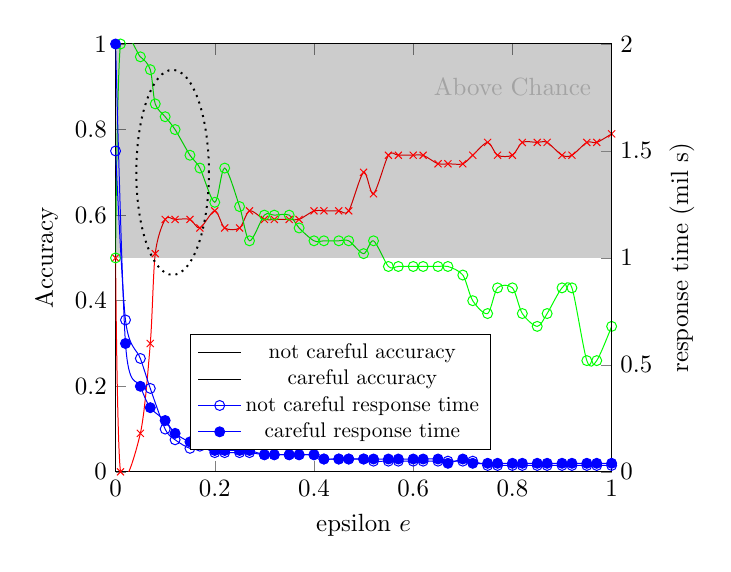
\begin{tikzpicture}[scale=0.9]
\pgfplotsset{
    scale only axis,
    scaled x ticks=base 10:0,
    xmin=0, xmax=1,
    legend style={at={(0.15,0.05)},anchor=south west},
    legend style={nodes={scale=0.85, transform shape}}
}

\begin{axis}[
  axis y line*=left,
  ymin=0, ymax=1,
  xlabel=epsilon $e$,
  ylabel=Accuracy,
]
\addplot[smooth,mark=x,red]
  coordinates{
    (0,0.5)
    (0.01,0)
    (0.05,0.09)
    (0.07,0.3)
    (0.08,0.51)
    (0.1,0.59)
    (0.12,0.59)
    (0.15,0.59)
    (0.17,0.57)
    (0.20,0.61)
    (0.22,0.57)
    (0.25,0.57)
    (0.27,0.61)
    (0.3,0.59)
    (0.32,0.59)
    (0.35,0.59)
    (0.37,0.59)
    (0.4,0.61)
    (0.42,0.61)
    (0.45,0.61)
    (0.47,0.61)
    (0.5,0.70)
    (0.52,0.65)
    (0.55,0.74)
    (0.57,0.74)
    (0.6,0.74)
    (0.62,0.74)
    (0.65,0.72)
    (0.67,0.72)
    (0.70,0.72)
    (0.72,0.74)
    (0.75,0.77)
    (0.77,0.74)
    (0.8,0.74)
    (0.82,0.77)
    (0.85,0.77)
    (0.87,0.77)
    (0.9,0.74)
    (0.92,0.74)
    (0.95,0.77)
    (0.97,0.77)
    (1,0.79)
}; \label{plot_one}

\addplot[smooth,mark=o,green]
  coordinates{
    (0,0.5)
    (0.01,1)
    (0.05,0.97)
    (0.07,0.94)
    (0.08,0.86)
    (0.1,0.83)
    (0.12,0.8)
    (0.15,0.74)
    (0.17,0.71)
    (0.20,0.63)
    (0.22,0.71)
    (0.25,0.62)
    (0.27,0.54)
    (0.3,0.6)
    (0.32,0.6)
    (0.35,0.6)
    (0.37,0.57)
    (0.4,0.54)
    (0.42,0.54)
    (0.45,0.54)
    (0.47,0.54)
    (0.5,0.51)
    (0.52,0.54)
    (0.55,0.48)
    (0.57,0.48)
    (0.6,0.48)
    (0.62,0.48)
    (0.65,0.48)
    (0.67,0.48)
    (0.70,0.46)
    (0.72,0.4)
    (0.75,0.37)
    (0.77,0.43)
    (0.8,0.43)
    (0.82,0.37)
    (0.85,0.34)
    (0.87,0.37)
    (0.9,0.43)
    (0.92,0.43)
    (0.95,0.26)
    (0.97,0.26)
    (1,0.34)
}; \label{plot_two}

% above chance level
\path[top color=black,bottom color=black,middle color=black, fill opacity=0.2] (0,0.5) rectangle (1,1) node[pos=.8] {Above Chance};

% region of interest
\coordinate (a) at (0.1, 0.6);
\coordinate (b) at (0.08,0.85);
\coordinate (c) at (0.15,0.55);
\coordinate (d) at (0.15,0.8);
    \node[ellipse, draw, thick, dotted, 
          fit=(a) (b) (c) (d)] {};
          
\end{axis}

\begin{axis}[
  axis y line*=right,
  axis x line=none,
  ymin=0, ymax=2,
  ylabel=response time (mil s)
]
\addlegendimage{/pgfplots/refstyle=plot_one}\addlegendentry{not careful accuracy}
\addlegendimage{/pgfplots/refstyle=plot_two}\addlegendentry{careful accuracy}
\addplot[smooth,mark=o,blue]
  coordinates{
    (0,1.5)
    (0.02,0.71)
    (0.05,0.53)
    (0.07,0.39)
    (0.1,0.2)
    (0.12,0.15)
    (0.15,0.11)
    (0.17,0.12)
    (0.20,0.09)
    (0.22,0.09)
    (0.25,0.09)
    (0.27,0.09)
    (0.3,0.08)
    (0.32,0.08)
    (0.35,0.08)
    (0.37,0.08)
    (0.4,0.08)
    (0.42,0.06)
    (0.45,0.06)
    (0.47,0.06)
    (0.5,0.06)
    (0.52,0.05)
    (0.55,0.05)
    (0.57,0.05)
    (0.6,0.05)
    (0.62,0.05)
    (0.65,0.05)
    (0.67,0.05)
    (0.70,0.05)
    (0.72,0.05)
    (0.75,0.03)
    (0.77,0.03)
    (0.8,0.03)
    (0.82,0.03)
    (0.85,0.03)
    (0.87,0.03)
    (0.9,0.03)
    (0.92,0.03)
    (0.95,0.03)
    (0.97,0.03)
    (1,0.03)
}; \addlegendentry{not careful response time}

\addplot[smooth,mark=*,blue]
  coordinates{
    (0,2)
    (0.02,0.6)
    (0.05,0.4)
    (0.07,0.3)
    (0.1,0.24)
    (0.12,0.18)
    (0.15,0.14)
    (0.17,0.14)
    (0.20,0.1)
    (0.22,0.1)
    (0.25,0.1)
    (0.27,0.1)
    (0.3,0.08)
    (0.32,0.08)
    (0.35,0.08)
    (0.37,0.08)
    (0.4,0.08)
    (0.42,0.06)
    (0.45,0.06)
    (0.47,0.06)
    (0.5,0.06)
    (0.52,0.06)
    (0.55,0.06)
    (0.57,0.06)
    (0.6,0.06)
    (0.62,0.06)
    (0.65,0.06)
    (0.67,0.04)
    (0.70,0.06)
    (0.72,0.04)
    (0.75,0.04)
    (0.77,0.04)
    (0.8,0.04)
    (0.82,0.04)
    (0.85,0.04)
    (0.87,0.04)
    (0.9,0.04)
    (0.92,0.04)
    (0.95,0.04)
    (0.97,0.04)
    (1,0.04)
}; \addlegendentry{careful response time}

\end{axis}

\end{tikzpicture}
  \caption{The evolution of the results for the epsilon}
  \label{fig:class_epsilon}
\end{figure}

\section{Human-Robot Applications}
\label{sec:robot}

- for the robot application the model chosen is the most successful model. the one that generalizes best for all people, all cups, and all datasets. 

- you should show a plot with the best model and the rate of change of epsilon. To see how sensitive epsilon is. 
\section{Conclusion}
\label{sec:conc}
The conclusion goes here.


% For peer review papers, you can put extra information on the cover
% page as needed:
% \ifCLASSOPTIONpeerreview
% \begin{center} \bfseries EDICS Category: 3-BBND \end{center}
% \fi
%
% For peerreview papers, this IEEEtran command inserts a page break and
% creates the second title. It will be ignored for other modes.
\IEEEpeerreviewmaketitle

% if have a single appendix:
%\appendix[Proof of the Zonklar Equations]
% or
%\appendix  % for no appendix heading
% do not use \section anymore after \appendix, only \section*
% \appendices
% \section{Proof of the First}
% you can choose not to have a title for an appendix
% if you want by leaving the argument blank
% \section{}
% results


% use section* for acknowledgment
\section*{Acknowledgment}

The authors would like to thank...

% Bibliography
\bibliographystyle{ieeetr}
\bibliography{IEEEabrv,references}



\end{document}


